\documentclass[tikz,border=2pt]{standalone}
\usepackage{amsmath,amssymb}
\usepackage{tikz}
\usetikzlibrary{arrows.meta}

\begin{document}
% Dimension = number of vectors in a basis: a line through 0 has dimension 1, a plane
% through 0 dimension 2, the whole of R^3 dimension 3.
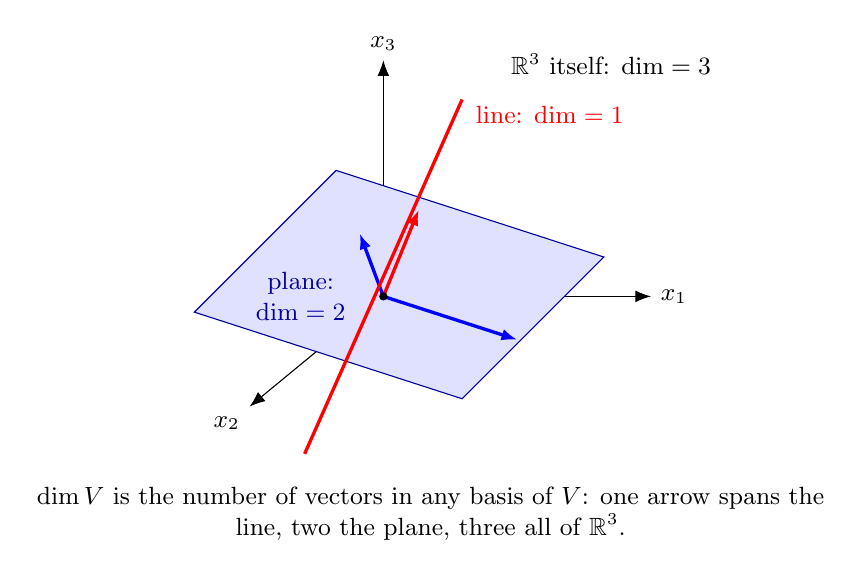
\begin{tikzpicture}[every node/.style={font=\small}, >={Latex[length=2mm]}]
	\draw[->] (0,0) -- (3.4,0) node[right] {$x_1$};
	\draw[->] (0,0) -- (0,3.0) node[above] {$x_3$};
	\draw[->] (0,0) -- (-1.7,-1.4) node[below left] {$x_2$};
	\fill[blue!12] (-2.4,-0.2) -- (1.0,-1.3) -- (2.8,0.5) -- (-0.6,1.6) -- cycle;
	\draw[blue!60!black] (-2.4,-0.2) -- (1.0,-1.3) -- (2.8,0.5) -- (-0.6,1.6) -- cycle;
	\draw[->, blue, very thick] (0,0) -- (1.7,-0.55);
	\draw[->, blue, very thick] (0,0) -- (-0.3,0.8);
	\node[blue!60!black, font=\small, align=center] at (-1.05,0.0) {plane:\\ $\dim=2$};
	\draw[red, very thick] (-1.0,-2.0) -- (1.0,2.5);
	\draw[->, red, very thick] (0,0) -- (0.45,1.1);
	\node[red, font=\small, anchor=west] at (1.05,2.3) {line: $\dim=1$};
	\node[anchor=west] at (1.5,2.95) {$\mathbb{R}^3$ itself: $\dim=3$};
	\fill (0,0) circle (1.5pt);
	\node[anchor=north, align=flush center, text width=10cm] at (0.6,-2.3) {$\dim V$ is the number of vectors in any basis of $V$: one arrow spans the line, two the plane, three all of $\mathbb{R}^3$.};
\end{tikzpicture}
\end{document}
